%=====================================================================
% IEEE Journal of Biomedical and Health Informatics (J-BHI) submission
% Port-Hamiltonian PINN Cardiac Digital Twin
% Compile in Overleaf: menu > IEEEtran (journal). Upload the figures/ folder.
%=====================================================================
\documentclass[journal]{IEEEtran}

\usepackage{amsmath,amssymb,amsfonts}
\usepackage{graphicx}
\usepackage{textcomp}
\usepackage{xcolor}
\usepackage[colorlinks=true,allcolors=blue]{hyperref}
\graphicspath{{figures/}}

\begin{document}

\title{Port-Hamiltonian Physics-Informed Neural Networks for Cardiac Hemodynamic Inference with Architecturally Guaranteed Energy Consistency}

\author{Kwanhyeong~Lee%
\thanks{K. Lee is an undergraduate student, Soonchunhyang University College of Medicine, Republic of Korea (e-mail: alex026376@sch.ac.kr).}%
\thanks{Manuscript submitted 2026.}}

\markboth{IEEE Journal of Biomedical and Health Informatics,~Vol.~XX, No.~X, 2026}%
{Lee: Port-Hamiltonian PINN with Guaranteed Energy Consistency}

\maketitle

\begin{abstract}
Cardiac digital twins aim to individualize cardiovascular care, but most approaches model anatomy, hemodynamics, and parameter inference in isolation and, in the machine-learning setting, give no guarantee that the physiological states they predict are physically admissible. We present a port-Hamiltonian physics-informed neural network (pH-PINN) framework that couples two components: (1)~a patient-anchored multi-structure reconstruction combining patient-specific CT segmentation with atlas-based registration (13 structures, 957{,}608 mesh elements); and (2)~a Windkessel-coupled PINN in which cardiovascular energy balance is imposed as an architectural inductive bias through a scalar port-Hamiltonian dissipation $R(x)=r_{\text{diss}}\,I$, with $r_{\text{diss}}$ fixed by the Windkessel characteristic impedance $Z_c$ rather than fit freely. Evaluated on the eICU ($n=3{,}991$) and MIMIC-IV ($n=5{,}851$) databases---keeping directly measured quantities strictly separate from surrogate-derived indices---the pH-PINN attained $R^2=0.975$ for cardiac output and $R^2=0.951$ for end-systolic elastance, distribution overlaps of $80.5\%$ (stroke volume) and $83.4\%$ (stroke work), and Pearson $r=0.916$ for systemic vascular resistance (measured via Swan--Ganz catheterization). The Windkessel--PINN bridge recovered physiologically consistent ventricular--arterial coupling ($E_a/E_{es}=0.60$) and a complete energy partition: gross mechanical efficiency $64.8\%$ (SW/PVA) and net efficiency $62.3\%$ once the port-Hamiltonian dissipation is subtracted ($E_{\text{diss}}=137$~mmHg$\cdot$mL per beat, $2.4\%$ of PVA). In a four-way ablation of matched-capacity models, the hard architectural constraints matched baseline predictive accuracy ($R^2\approx0.97$) while guaranteeing physically valid internal states by construction, whereas identical-capacity unconstrained baselines produced negative energies and non-positive-semidefinite dissipation in up to $100\%$ of test cases. The framework supports non-invasive cardiac digital twins whose internal states respect fundamental energy constraints by construction.
\end{abstract}

\begin{IEEEkeywords}
Physics-informed neural network, cardiac digital twin, port-Hamiltonian system, ventricular--arterial coupling, hemodynamic inference, patient-anchored hybrid geometry, energy dissipation.
\end{IEEEkeywords}

\section{Introduction}\label{sec:intro}
\IEEEPARstart{C}{ardiac} digital twins---computational replicas of an individual patient's heart that integrate anatomical, hemodynamic, and electrophysiological data---are an emerging technology in cardiovascular medicine \cite{corral2020}. By allowing therapies to be tested \emph{in silico} before clinical use, they can improve treatment planning for heart failure, valvular disease, and cardiac surgery. Building a clinically useful twin, however, requires solving three coupled problems: faithful anatomical reconstruction, accurate hemodynamic modeling, and reliable parameter inference from non-invasive measurements.

Existing methods typically address these problems separately. Anatomical pipelines extract cardiac geometry from imaging but seldom feed downstream hemodynamic analysis; computational fluid dynamics resolves intracardiac flow in high fidelity but at hours of computation per cycle, limiting bedside use; and machine-learning surrogates accelerate inference but often lack the physical constraints needed for physiologically plausible predictions outside the training distribution \cite{greener2022}.

Physics-informed neural networks (PINNs) offer a principled way to combine data-driven flexibility with physical fidelity \cite{raissi2019}: by embedding governing equations as soft penalties in the loss, they can learn solutions that respect conservation laws even from sparse or noisy clinical data. Yet cardiac PINNs typically enforce individual ordinary differential equations---most often the time-varying elastance model---without exploiting the deeper geometric structure of Hamiltonian mechanics that governs energy exchange in a dissipative system. The port-Hamiltonian $J$--$R$ structure is well established in cardiovascular engineering---for example, in the passivity-based control of cardiac assist devices \cite{hammoud2026}---but we adopt it here as an architectural prior for non-invasive inference rather than for device control.

In this work we propose a port-Hamiltonian PINN (pH-PINN) that enforces energy balance through the port-Hamiltonian structure~\eqref{eq:ph}, in which $J(x)=-J^{\top}(x)$ is the skew-symmetric interconnection encoding energy-conserving dynamics, $R(x)\succeq 0$ is the positive semidefinite dissipation capturing viscous and viscoelastic losses, $H$ is the total (kinetic plus potential) energy, and $g(x)u$ is the external input from cardiac contraction. Rather than demanding strict conservation ($dH/dt=0$, which is non-physical for a dissipative circulation), the architecture guarantees the passivity inequality $dH/dt\le y^{\top}u$ pointwise by emitting a positive semidefinite $R(x)$, together with a non-negative energy partition $H=T+V$. We embed this pH-PINN in a modular digital-twin pipeline that couples (i)~a patient-anchored reconstruction assembling 13 cardiac structures ($957{,}608$ mesh elements) across three provenance tiers to (ii)~a Windkessel--PINN bridge that maps hemodynamic waveforms to lumped-parameter indices ($E_a$, $E_{es}$, coupling ratio) within the same energy-balance framework, with the dissipation strength fixed by the Windkessel characteristic impedance.

We evaluate the framework on 9{,}842 critically ill patients from two independent ICU databases (eICU and MIMIC-IV) and separate directly measured quantities (cardiac output by thermodilution, systemic vascular resistance by Swan--Ganz catheterization) from surrogate-derived indices ($E_{es}$, mechanical efficiency). This distinction, often blurred in the PINN literature \cite{karniadakis2021,kissas2020}, determines how much validation weight each result carries.

% Graphical abstract (Figure1_GraphicalAbstract.png) submitted as a separate file; not counted toward the page limit.

\section{Methods}\label{sec:methods}

\subsection{Patient-Anchored Multi-Structure Anatomical Reconstruction}\label{sec:anat}
The anatomical reconstruction provides the geometric context of the pipeline; the hemodynamic inference evaluated in Section~\ref{sec:results} is lumped-parameter (0D) and does not consume the mesh, since the ICU cohorts have no paired volumetric imaging. The pipeline employs a three-tier patient-specificity hierarchy (Supplementary Table~S2) to assemble a 13-structure cardiac geometry, following the hybrid atlas-registration approach of Zhang \emph{et al.} \cite{zhang2012} and Kong \emph{et al.} \cite{kong2023}. This is consistent with the view that practical cardiac digital twins combine patient-derived imaging data with population-level anatomical priors \cite{corral2020,rodero2021,hoogendoorn2013}.

\emph{Tier 1 (Patient-specific):} The primary left ventricular (LV) surface was directly segmented from the MM-WHS (Multi-Modality Whole Heart Segmentation) Challenge CT dataset (Case 1009) using label-based extraction, yielding 166{,}936 triangular mesh elements \cite{zhuang2019}.

\emph{Tier 2 (Patient-adapted):} Papillary muscles were separated from the combined myocardial segmentation using $K$-means clustering (anterolateral: 122{,}314 elements; posteromedial: 131{,}606 elements), and wall-thickness distributions were derived from the patient CT (mean $6.8\pm2.1$~mm).

\emph{Tier 3 (Atlas-registered):} Six additional structures (left atrial appendage, right ventricle, coronary arteries, pulmonary veins, pulmonary artery, right atrium) were extracted from the STACOM2025 whole-heart atlas. Coordinate registration between MM-WHS and STACOM reference frames used iterative closest point (ICP) alignment with the LV surface as reference (mean registration distance $0.35$--$0.58$, compared to target $<0.15$; see Limitations).

\emph{Parametrically generated:} Valve geometries (mitral and aortic) were generated from published dimensions: the mitral valve followed Kunzelman \emph{et al.} \cite{kunzelman1994} (annulus diameter 30~mm, leaflet height 15~mm), and the aortic valve followed Thubrikar \emph{et al.} \cite{thubrikar1981} (23~mm annulus). Chordae tendineae followed Lam \emph{et al.} \cite{lam1970} with 12 primary chordae per papillary muscle. The final assembly was validated across 20 MM-WHS cases to establish population-level anatomical statistics (chamber volumes, wall thickness, and assembly inventory; Supplementary Material, Fig.~S1 and Table~S2).

\subsection{Port-Hamiltonian Physics-Informed Neural Network}\label{sec:pinn}
The pH-PINN architecture consists of a fully connected neural network with 61{,}169 trainable parameters that maps non-invasive hemodynamic features (heart rate, blood pressure, echocardiographic measurements) to physiological parameters ($E_{es}$, $E_{ed}$, $E_a$, ventricular--arterial coupling ratio, end-diastolic pressure, mechanical efficiency, relaxation time constant $\tau$).

\emph{State variables and energy heads.} The encoder maps the $11$ non-invasive input features to the port-Hamiltonian state $x=(q,p)\in\mathbb{R}^{5}$---generalized chamber volumes $q=(V_{LV},V_{LA},V_{art})$ and inertance-scaled valve-flow momenta $p=(p_{mv},p_{ao})$---plus auxiliary elastances ($E_{es}$, $E_{ed}$, $V_0$, $\tau$). Separate non-negative heads emit the potential $V(q)=\mathrm{softplus}(f_V(q))$ and the kinetic energy $T(q,p)=\tfrac{1}{2}p^{\top}M^{-1}(q)p$ ($M^{-1}(q)\succ0$), so that $T,V\ge0$ and $H=T+V$ hold \emph{by construction}. Input features, state bounds, per-head definitions, and an architecture schematic appear in Supplementary Section~S3 (Fig.~S2, Table~S3). The network performs \emph{per-beat} (steady-state) inference: it maps a patient's non-invasive feature vector to the state $x=(q,p)$ and the associated energetics for a representative cardiac cycle. It does not take time as an input and does not integrate a trajectory; all derivatives are taken with respect to the state, not with respect to time.

\emph{Port-Hamiltonian formulation.} The cardiovascular system is inherently dissipative: viscous losses in blood flow, myocardial viscoelasticity, and valve turbulence all dissipate energy. A pure Hamiltonian formulation ($dH/dt=0$) would be non-physical. We therefore adopt the port-Hamiltonian framework \cite{vanderschaft2014}, which decomposes the system dynamics into energy-conserving ($J$) and energy-dissipating ($R$) components:
\begin{equation}\label{eq:ph}
\dot{x} = \left[J(x) - R(x)\right]\frac{\partial H}{\partial x} + g(x)\,u
\end{equation}
\begin{equation}\label{eq:balance}
\frac{dH}{dt} = -\left(\frac{\partial H}{\partial x}\right)^{\!\top}\! R(x)\left(\frac{\partial H}{\partial x}\right) + y^{\top}u \;\le\; y^{\top}u
\end{equation}
Equation~\eqref{eq:balance} encodes the energy balance: the rate of change of the Hamiltonian equals the dissipated power (first term, always non-positive) plus the supplied power. Because the network emits $R(x)\succeq0$ by construction, the quadratic form $(\partial H/\partial x)^{\top}R(\partial H/\partial x)$ is non-negative for every sample, so the passivity inequality $dH/dt\le y^{\top}u$ in~\eqref{eq:balance} holds \emph{structurally} and does not have to be imposed by a penalty. Given a state estimate, the instantaneous rate $\dot{x}$ is evaluated from~\eqref{eq:ph}; because the present model performs per-beat inference on cross-sectional data, $\dot{x}$ is not compared against a measured time derivative, and no time-marching residual is minimized.

\emph{Dissipation parameterization.} We parameterize $R(x)=r_{\text{diss}}\,I$ as a scalar (isotropic) dissipation matrix, where $r_{\text{diss}}$ is calibrated from the Windkessel characteristic impedance $Z_c$ ($=R_1$) \cite{westerhof2009}, scaled by the systolic ejection duty cycle:
\begin{equation}\label{eq:rdiss}
r_{\text{diss}} = R_1 \times \left(T_{\text{sys}} / T_{\text{cycle}}\right)
\end{equation}
This grounds the dissipation in a measurable hemodynamic quantity: $Z_c$ represents the resistive component of aortic input impedance, capturing wave reflection and viscous losses at the aortic root---exactly the energy dissipation that a port-Hamiltonian cardiovascular model should capture \cite{westerhof2009}. For the nominal case ($R_1=0.072$, HR${}=75$, $T_{\text{sys}}=0.285$~s), $r_{\text{diss}}=0.026$~mmHg$\cdot$s/mL, consistent with the expected physiological range of $0.01$--$0.05$ for normal cardiac function. Learning a state-dependent $R(x)$ from clinical data (e.g., Doppler-derived turbulence kinetic energy) is a natural extension, but is outside the scope of this initial validation.

The training objective combines data fidelity with the algebraic energy constraints that remain after the architectural ones:
\begin{equation}\label{eq:ltotal}
L_{\text{total}} = L_{\text{data}} + \lambda_H\left(L_{\text{part}} + L_{\text{pos}}\right) + \lambda_{\text{PSD}}\,L_{\text{PSD}}
\end{equation}
where $L_{\text{data}}$ is the mean squared error over the clinical and energetic targets, $L_{\text{part}}=\lVert H-(T+V)\rVert^{2}$ is the Hamiltonian partition consistency, $L_{\text{pos}}=\lVert\mathrm{ReLU}(-T)\rVert^{2}+\lVert\mathrm{ReLU}(-V)\rVert^{2}$ penalizes negative energies, and $L_{\text{PSD}}$ penalizes negative eigenvalues of $R$. In the hard-constrained architecture all three physics terms are already satisfied by construction, so they act as numerical safeguards rather than as active constraints; they become active only in the unconstrained and soft-constrained ablation variants (Section~\ref{sec:ablation}). All computations use single-precision (float32) arithmetic. The network was trained for 150 epochs with the AdamW optimizer and a cosine learning-rate schedule, converging at epoch~115 (best validation loss).

\subsection{Windkessel--PINN Bridge}\label{sec:wk}
The Windkessel--PINN bridge connects lumped-parameter hemodynamics to the pH-PINN for calibrated parameter estimation. A three-element Windkessel model (proximal resistance $R_1$, distal resistance $R_2$, arterial compliance $C$) is fitted to hemodynamic waveforms. The resulting Windkessel parameters, combined with cardiac-function indices from pressure--volume (PV) loop analysis (Section~\ref{sec:pv}), are fed into the pH-PINN.

\subsubsection{PV loop energy partition with dissipation}\label{sec:pv}
Following the Suga--Sagawa framework \cite{suga1974}, stroke work (SW) was computed as the area under the arterial elastance ($E_a$) line on the PV diagram:
\begin{equation}\label{eq:sw}
\text{SW} = \tfrac{1}{2}\, E_a \,\text{SV}^2
\end{equation}
Potential energy (PE) was computed from the end-systolic pressure--volume relation (ESPVR):
\begin{equation}\label{eq:pe}
\text{PE} = \tfrac{1}{2}\, E_{es}\,(V_{es} - V_0)^2
\end{equation}
Dissipation energy per beat was computed from the port-Hamiltonian energy balance~\eqref{eq:balance}:
\begin{equation}\label{eq:ediss}
E_{\text{diss}} = r_{\text{diss}} \times \text{SV} \times \bar{P}_{\text{sys}}
\end{equation}
where $\bar{P}_{\text{sys}}$ is the mean systolic pressure. Net stroke work is $\text{SW}_{\text{net}}=\text{SW}-E_{\text{diss}}$. The PV area ($\text{PVA}=\text{SW}+\text{PE}$) represents total mechanical energy per beat. Dual efficiency metrics are reported: gross efficiency $\eta_{\text{gross}}=\text{SW}/\text{PVA}$ (Suga--Sagawa \cite{suga1974}) and net efficiency $\eta_{\text{net}}=(\text{SW}-E_{\text{diss}})/\text{PVA}$, which accounts for the port-Hamiltonian dissipation.

\subsection{Validation Strategy and Cohorts}\label{sec:val}
External validation used two independent ICU databases: the eICU Collaborative Research Database ($n=3{,}991$) and MIMIC-IV ($n=5{,}851$) \cite{johnson2023,johnson2016,pollard2018}. To avoid overstating validation strength, we explicitly categorize the validation variables by measurement provenance (Table~\ref{tab:prov}):

\emph{Directly measured (gold standard):} Cardiac output (CO) via thermodilution, systemic vascular resistance (SVR) computed from directly measured CO, MAP, and CVP via Swan--Ganz catheterization, and pulmonary artery wedge pressure (PAWP).

\emph{Surrogate-derived (estimated):} End-systolic elastance ($E_{es}$), arterial elastance ($E_a$), stroke work, ventricular--arterial coupling ratio, and mechanical efficiency. These are computed from directly measured hemodynamics using validated surrogate formulas (single-beat estimation; $P_{es}\approx0.9\,\text{SBP}$) \cite{chen2001}, not from invasive catheter-based PV loop recordings.

This distinction matters: agreement between pH-PINN predictions and surrogate-derived indices demonstrates that the PINN reproduces the same hemodynamic relationships encoded in the surrogate formulas, not that it matches independent gold-standard measurements for those specific parameters.

\subsection{Ablation Design}\label{sec:ablation}
To test whether the port-Hamiltonian structure contributes beyond raw network capacity, we compared four matched-capacity models on the same 13-target cardiac energetics dataset ($n=5{,}851$): (A)~the pH-PINN with \emph{hard} architectural constraints---softplus non-negativity of kinetic ($T$) and potential ($V$) energy, $H=T+V$ by construction, and a Cholesky-parameterized dissipation matrix $R=LL^{\top}\succeq0$; (B)~a vanilla multilayer perceptron with no physics structure; (C)~a no-structure PINN with encoder/decoder topology identical to (A) but \emph{without} the hard constraints; and (D)~a soft-constraint PINN that instead penalizes constraint violations in the loss. Models (A), (C), and (D) share an identical $73{,}773$-parameter architecture---a capacity-matched re-implementation of the production pH-PINN (Section~\ref{sec:pinn}, $61{,}169$ parameters) used solely for this comparison, so that the four variants differ only in their constraints and not in capacity. All variants were trained for 80 epochs (AdamW, cosine learning-rate schedule) and evaluated over three random seeds; we report the mean $\pm$ standard deviation. We report predictive accuracy (mean $R^2$ over 13 targets) on a random $80/20$ split and under a temporal (median-echo-date) split, together with physical-validity diagnostics on the held-out set: the $H=T+V$ consistency error, the number of cases with negative $T$ or $V$, and the number with a non-positive-semidefinite (non-PSD) dissipation matrix.

\subsection{Model Applicability and Target Population}\label{sec:pop}
The present framework targets patients requiring \emph{LV-centric pump function assessment}. This scope reflects the three-tier patient-specificity hierarchy (Supplementary Table~S2): only the LV surface is directly patient-specific (Tier~1), while other structures are atlas-registered (Tier~3) and therefore contribute geometric context but not patient-specific hemodynamic constraints.

\emph{Inclusion criteria:} Adult patients ($\ge 18$~years) with preserved or reduced LV systolic function undergoing echocardiographic or catheter-based hemodynamic assessment. Applicable conditions include heart failure with reduced ejection fraction (HFrEF), heart failure with preserved ejection fraction (HFpEF), hypertensive heart disease, and ischemic cardiomyopathy.

\emph{Exclusion criteria:} (1)~Hemodynamically significant valvular disease (moderate or greater mitral/aortic regurgitation or stenosis), as the Windkessel model assumes unidirectional aortic outflow without regurgitant fraction. (2)~Significant right ventricular pathology (pulmonary hypertension, RV infarction, arrhythmogenic RV cardiomyopathy), as the RV is Tier~3 atlas-registered. (3)~Congenital heart disease (septal defects, single-ventricle physiology), which violates the two-chamber (LV--aorta) Windkessel assumption. (4)~Mechanical circulatory support (LVAD, ECMO, IABP), which fundamentally alters the PV relationship. These criteria ensure the model operates within the domain where its physics-based assumptions are valid and its patient-specific data inputs are most informative.

\section{Results}\label{sec:results}

\subsection{pH-PINN Training and Convergence}\label{sec:train}
The pH-PINN converged after 115 epochs, achieving a final validation loss of 0.074 and training loss of 0.073 (Fig.~\ref{fig:training}(A)). The model achieved $R^2=0.975$ for cardiac output prediction and $R^2=0.951$ for end-systolic elastance ($E_{es}$) estimation (Fig.~\ref{fig:training}(B)). The Hamiltonian partition consistency error, $L_{\text{part}}=\lVert H-(T+V)\rVert^{2}$, remained at the rounding level of single-precision arithmetic throughout training, decreasing from $5.2\times10^{-15}$ at epoch~1 to $2.5\times10^{-15}$ at convergence (epoch~115), with a final value of $2.8\times10^{-15}$ at epoch~150 (Fig.~\ref{fig:training}(C)). Because $H$ is formed as $T+V$ inside the network, this quantity is expected to sit at float32 machine precision (a mean squared error of ${\sim}10^{-15}$ corresponds to a root-mean-square deviation of ${\sim}3\times10^{-8}$, i.e. the float32 epsilon); it therefore verifies the \emph{algebraic} energy partition and the absence of numerical drift, and should not be read as a residual of the dynamic energy balance~\eqref{eq:balance}, which is instead guaranteed structurally by $R(x)\succeq0$. The dissipation contribution is quantified separately in Section~\ref{sec:wkpv}.

Per-parameter test accuracy was high across all seven targets: $E_{es}$ ($R^2=0.984$), $E_{ed}$ ($R^2=0.991$), $E_a$ ($R^2=0.978$), ventricular--arterial coupling ($R^2=0.982$), end-diastolic pressure ($R^2=0.957$), mechanical efficiency ($R^2=0.982$), and relaxation time constant $\tau$ ($R^2=0.983$); full per-parameter details are in Supplementary Table~S1.

\begin{figure*}[!t]
\centering
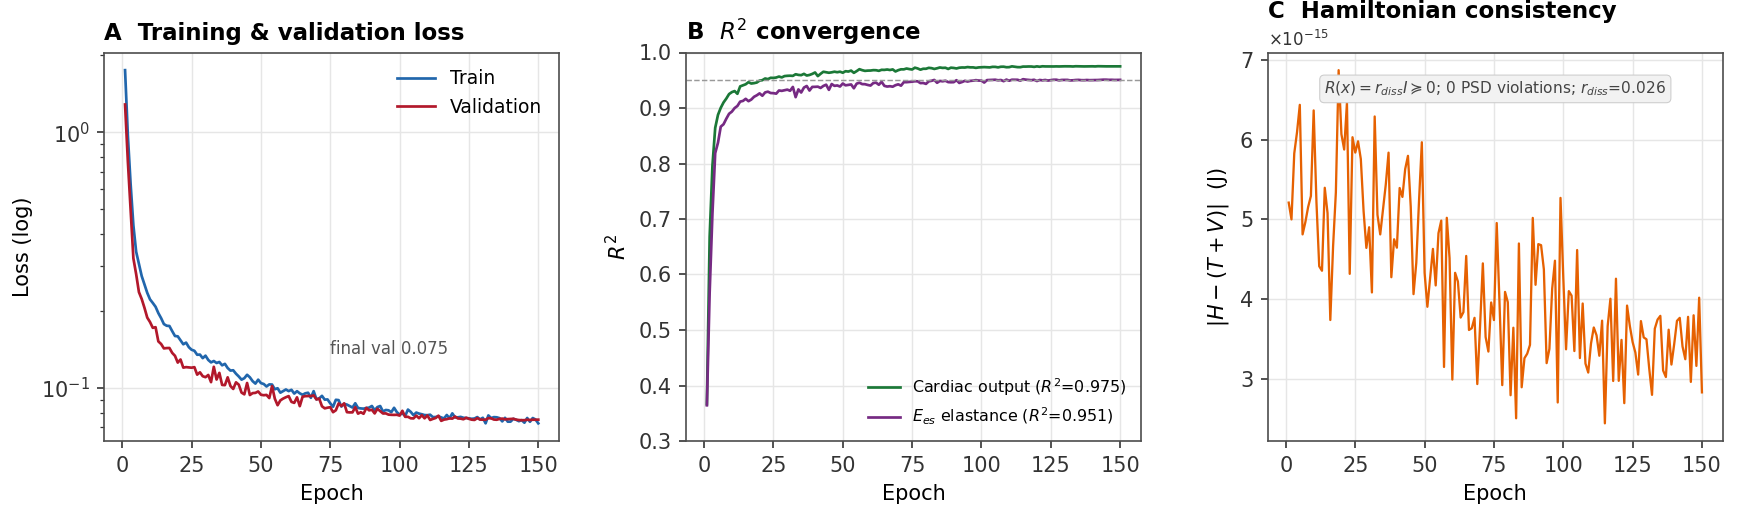
\includegraphics[width=0.98\textwidth]{Fig2_training_preview.png}
\caption{pH-PINN training convergence. (A)~Training and validation loss over 150 epochs (log scale). (B)~$R^2$ convergence for cardiac output (green) and $E_{es}$ (purple). (C)~Hamiltonian partition consistency error $\lVert H-(T+V)\rVert^{2}$, which stays at float32 rounding level (${\sim}3\times10^{-15}$) because $H=T+V$ holds by construction; no non-PSD dissipation matrices occurred. Model: 61{,}169 parameters, best epoch 115.}
\label{fig:training}
\end{figure*}

\subsection{Ablation: Physics Constraints as Inductive Bias}\label{sec:ablres}
Table~\ref{tab:ablation} and Fig.~\ref{fig:ablation} summarize the ablation. Across three seeds, all four models reached comparable predictive accuracy---mean $R^2$ of $0.972\pm0.001$ (hard), $0.972\pm0.001$ (vanilla MLP), $0.973\pm0.000$ (no-structure), and $0.970\pm0.001$ (soft) on the random split; the largest between-model difference ($0.003$) is on the order of the seed-to-seed standard deviation, and the ordering is preserved under a temporal (median-echo-date) split ($0.968$--$0.971$). Predictive accuracy is therefore \emph{not} the discriminating axis (Fig.~\ref{fig:ablation}(A)).

Physical validity is the discriminating factor. The hard-constrained pH-PINN~(A) produced zero violations by construction: $H=T+V$ to machine precision ($1.3\times10^{-15}$), no negative energies, and no non-PSD dissipation matrices across all $1{,}171$ held-out cases. By contrast, the same-capacity no-structure PINN~(C)---an identical $73{,}773$-parameter topology whose $R^2$ matches (A) to within seed variability---produced (seed mean) $689$ negative kinetic-energy cases, $514$ negative potential-energy cases, and a non-PSD dissipation matrix in \emph{every} one of the $1{,}171$ test cases (Fig.~\ref{fig:ablation}(B)). The vanilla MLP~(B) violated $H=T+V$ by $O(1)$ and produced ${\sim}800$ negative-energy cases. The soft-constraint model~(D) recovered validity on this in-distribution test set, but only through a hand-tuned penalty weight, with no out-of-distribution guarantee and a small accuracy cost. The port-Hamiltonian structure therefore acts as an architectural inductive bias that yields physically valid internal states \emph{at no accuracy cost and without penalty tuning}, which is the property required for a trustworthy physiological digital twin.

\begin{figure*}[!t]
\centering

\includegraphics[width=0.98\textwidth]{Fig6_ablation_preview.png}
\caption{Ablation study: physics constraints as architectural inductive bias. (A)~Mean $R^2$ over 13 targets on the random split (three seeds; bars show mean, error bars SD)---predictive accuracy is comparable across all four matched-capacity models. (B)~Physical-validity violations on the $1{,}171$-case held-out set (seed mean): negative kinetic energy ($T<0$), negative potential energy ($V<0$), and non-PSD dissipation ($R\not\succeq0$). Hard architectural constraints (A) guarantee zero violations; the soft-constraint model (D) reaches zero only via a tuned penalty; unconstrained models (B, C) violate physical validity in hundreds to all test cases despite matched accuracy.}
\label{fig:ablation}
\end{figure*}

\begin{table*}[!t]
\caption{Ablation: Predictive Accuracy vs. Physical Validity Across Four Matched-Capacity Models (Random Split, 3 Seeds; $1{,}171$ Held-Out Cases)}
\label{tab:ablation}
\centering
\footnotesize
\begin{tabular}{llccccccl}
\hline
\textbf{Model} & \textbf{Params} & \textbf{$R^2$ (rand.)} & \textbf{$R^2$ (temp.)} & \textbf{$H{=}T{+}V$ MSE} & \textbf{$T<0$} & \textbf{$V<0$} & \textbf{$R\not\succeq0$} & \textbf{Validity}\\
\hline
A: pH-PINN (hard) & 73{,}773 & $0.972{\pm}0.001$ & 0.970 & $1.3\times10^{-15}$ & 0 & 0 & 0 & guaranteed\\
B: Vanilla MLP & 111{,}885 & $0.972{\pm}0.001$ & 0.969 & $1.3\times10^{0}$ & 800 & 895 & n/a & none\\
C: No-structure PINN & 73{,}773 & $0.973{\pm}0.000$ & 0.971 & $6.8\times10^{-16}$ & 689 & 514 & 1171 & none\\
D: Soft-constraint PINN & 73{,}773 & $0.970{\pm}0.001$ & 0.968 & $8.1\times10^{-17}$ & 0 & 0 & 0 & via penalty\\
\hline
\end{tabular}

\vspace{2pt}
\begin{minipage}{\textwidth}
\footnotesize $R^2$ (rand.) is mean $\pm$ SD over three seeds; violation counts are seed means on the $1{,}171$-case held-out set. Models A, C, and D share an identical $73{,}773$-parameter architecture, isolating the effect of the physics constraints. All models reach comparable predictive accuracy; only the hard-constrained model (A) guarantees physical validity by construction. ``n/a'': the vanilla MLP has no explicit dissipation matrix.
\end{minipage}
\end{table*}

\begin{table*}[!t]
\caption{Validation Variable Provenance: Directly Measured vs. Surrogate-Derived Parameters}
\label{tab:prov}
\centering
\footnotesize
\begin{tabular}{llll}
\hline
\textbf{Parameter} & \textbf{Provenance} & \textbf{Measurement Method} & \textbf{Validation Strength}\\
\hline
CO (L/min) & Direct & Thermodilution (Swan--Ganz) & Gold standard\\
SVR (dyn$\cdot$s/cm$^5$) & Direct & MAP, CO, CVP (all Swan--Ganz) & Gold standard\\
PAWP (mmHg) & Direct & Pulmonary artery catheter & Gold standard\\
SV (mL) & Semi-direct & CO/HR & Strong (derived from direct)\\
$E_a$ (mmHg/mL) & Surrogate & $P_{es}/\text{SV}\approx(0.9\times\text{SBP})/\text{SV}$ & Internal consistency\\
$E_{es}$ (mmHg/mL) & Surrogate & Single-beat estimation & Internal consistency\\
SW (g$\cdot$m) & Surrogate & MAP $\times$ SV $\times$ 0.0136 & Internal consistency\\
Mech. Eff. (\%) & Surrogate & SW/PVA (Suga model) & Internal consistency\\
\hline
\end{tabular}

\vspace{2pt}
\begin{minipage}{\textwidth}
\footnotesize Direct $=$ measured by invasive catheter; Surrogate $=$ estimated from directly measured hemodynamics using validated formulas; Internal consistency $=$ PINN reproduces surrogate-formula relationships, not independent gold-standard measurements.
\end{minipage}
\end{table*}

% Anatomical-reconstruction results (chamber volumes, wall thickness, assembly inventory) moved to Supplementary Material (Fig. S1, Table S2) to meet the page limit.

\subsection{Hemodynamic Cross-Validation}\label{sec:xval}
Cross-validation between eICU ($n=3{,}991$) and MIMIC-IV ($n=5{,}851$) showed agreement across the key hemodynamic parameters (Fig.~\ref{fig:xval}). Distribution overlaps were $80.5\%$ for stroke volume (SV), $72.5\%$ for arterial elastance ($E_a$), $83.4\%$ for stroke work (SW), and $65.2\%$ for cardiac output (CO). The lower overlap for CO reflects known systematic differences between the two databases in CO measurement methodology.

\emph{Directly measured parameter validation:} Bland--Altman analysis \cite{blandaltman1986} for SVR---computed entirely from Swan--Ganz catheter-derived CO, MAP, and CVP---yielded Pearson $r=0.916$ ($p<10^{-300}$) with a bias of $175.5$~dyn$\cdot$s/cm$^5$ and limits of agreement from $-98.2$ to $449.3$~dyn$\cdot$s/cm$^5$ (Fig.~\ref{fig:xval}(B)). The mean absolute error was $182.7$~dyn$\cdot$s/cm$^5$ across 2{,}704 paired measurements. This represents the strongest validation evidence, as SVR is derived entirely from directly measured hemodynamic quantities.

\emph{Surrogate-derived parameter agreement:} Distribution overlaps for surrogate-derived parameters ($E_a$: $72.5\%$, SW: $83.4\%$) indicate that the pH-PINN reproduces the hemodynamic relationships embedded in established surrogate formulas, providing internal consistency rather than independent ground-truth validation.

\begin{figure*}[!t]
\centering
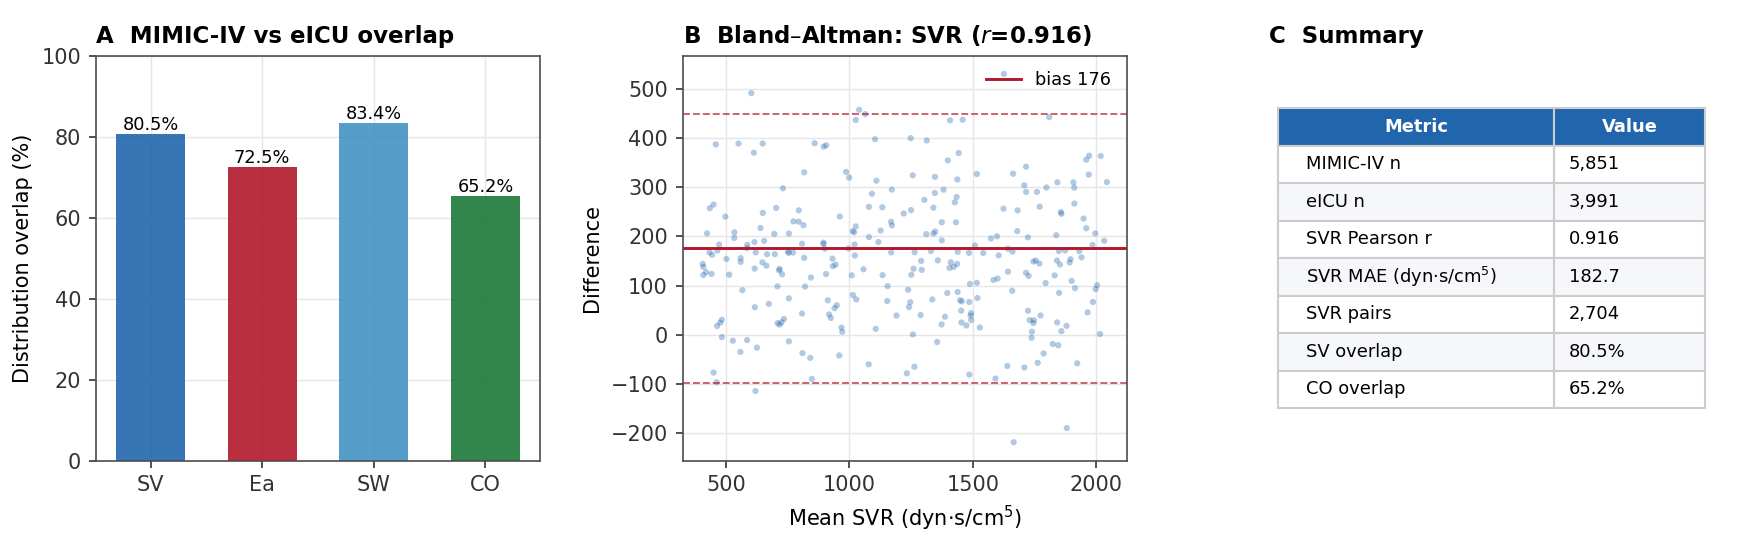
\includegraphics[width=0.98\textwidth]{Fig4_validation_preview.png}
\caption{Hemodynamic cross-validation. (A)~Distribution overlap between MIMIC-IV and eICU for stroke volume, arterial elastance, stroke work, and cardiac output. (B)~Bland--Altman plot for SVR (directly measured via Swan--Ganz; Pearson $r=0.916$). (C)~Summary metrics. Parameters are categorized by measurement provenance (Table~\ref{tab:prov}).}
\label{fig:xval}
\end{figure*}

\subsection{Windkessel--PINN Integration and PV Loop Analysis}\label{sec:wkpv}
The Windkessel model fitted to hemodynamic waveforms yielded physiologically plausible parameters: $R_1=0.072$~mmHg$\cdot$s/mL, $R_2=1.128$~mmHg$\cdot$s/mL, and $C=1.750$~mL/mmHg (Fig.~\ref{fig:pvloop}(B)). These corresponded to a mean aortic pressure of $104.5$~mmHg at 75~bpm with stroke volume 70~mL and cardiac output 5.25~L/min.

The pH-PINN integration with port-Hamiltonian dissipation yielded $E_{es}=2.5$~mmHg/mL, $E_a=1.50$~mmHg/mL, and a ventricular--arterial coupling ratio ($E_a/E_{es}$) of 0.60, indicating efficient coupling within the physiological range of $0.5$--$1.2$ (Fig.~\ref{fig:pvloop}(A)). The dissipation parameter $r_{\text{diss}}=0.026$~mmHg$\cdot$s/mL, estimated from $Z_c$ via~\eqref{eq:rdiss}, falls within the expected range for normal cardiac function ($0.01$--$0.05$).

PV loop energy partition following the Suga--Sagawa framework~(\ref{eq:sw})--(\ref{eq:pe}) with port-Hamiltonian dissipation~\eqref{eq:ediss} showed stroke work $\text{SW}=3{,}675$~mmHg$\cdot$mL ($0.49$~J) and potential energy $\text{PE}=2{,}000$~mmHg$\cdot$mL, yielding $\text{PVA}=5{,}675$~mmHg$\cdot$mL. Dissipation energy per beat was $E_{\text{diss}}=137.1$~mmHg$\cdot$mL ($2.4\%$ of PVA), yielding net stroke work $\text{SW}_{\text{net}}=3{,}538$~mmHg$\cdot$mL. Dual efficiency metrics: gross efficiency (SW/PVA) $=64.8\%$, net efficiency $((\text{SW}-E_{\text{diss}})/\text{PVA})=62.3\%$ (Fig.~\ref{fig:pvloop}(C)). The gross efficiency is consistent with the theoretical prediction for optimal coupling ($E_a/E_{es}=0.6$): $\eta = 1/(1 + \text{PE}/\text{SW}) = 64.8\%$ \cite{suga1974}.

\begin{figure*}[!t]
\centering

\includegraphics[width=0.98\textwidth]{Fig5_pvloop_preview.png}
\caption{PV loop and port-Hamiltonian energy balance. (A)~Reconstructed LV pressure--volume loop with ESPVR ($E_{es}=2.5$~mmHg/mL) and end-diastolic pressure--volume relation (EDPVR) lines. (B)~Windkessel parameters ($R_1,R_2,C$) and dissipation parameter $r_{\text{diss}}$ (red; estimated from $Z_c$ via~\eqref{eq:rdiss}). (C)~PV-area decomposition: stroke work (SW $=3{,}675$~mmHg$\cdot$mL, gross efficiency $64.8\%$), dissipation energy ($E_{\text{diss}}=137.1$~mmHg$\cdot$mL, $2.4\%$), net stroke work ($\text{SW}_{\text{net}}=3{,}538$~mmHg$\cdot$mL, net efficiency $62.3\%$), and potential energy (PE $=2{,}000$~mmHg$\cdot$mL).}
\label{fig:pvloop}
\end{figure*}

\section{Discussion}\label{sec:discussion}
We have presented a modular cardiac digital-twin framework that integrates anatomical reconstruction, Windkessel modeling, and a port-Hamiltonian PINN with scalar dissipation for hemodynamic inference. We discuss three contributions and their limitations.

\emph{Port-Hamiltonian energy balance with dissipation as inductive bias.} The pH-PINN's enforcement of energy balance through the port-Hamiltonian structure~(\ref{eq:ph})--(\ref{eq:balance}) imposes a geometric constraint that is stronger than individual equation residuals. The scalar dissipation parameterization $R(x)=r_{\text{diss}}\,I$, with $r_{\text{diss}}$ estimated from the Windkessel characteristic impedance $Z_c$ \cite{westerhof2009}, transforms the energy balance from a self-consistency check into a physically grounded constraint: the dissipation energy of $137.1$~mmHg$\cdot$mL per beat ($2.4\%$ of PVA) represents actual viscous losses at the aortic root, not a numerical artifact. The net mechanical efficiency ($62.3\%$) provides a more physically complete metric than gross efficiency alone. Standard PINNs that enforce time-varying elastance ODEs can overfit to the training cohort's hemodynamic regime; the Hamiltonian constraint penalizes solutions that are kinematically valid but energetically implausible. The ablation (Section~\ref{sec:ablres}) quantifies this: an identical-capacity network without the hard constraints matches predictive accuracy yet produces physically impossible internal states---negative kinetic/potential energies and non-PSD dissipation---in the majority of test cases, whereas the constrained architecture guarantees validity at no accuracy cost.

\emph{Modular pipeline architecture.} Most cardiac digital-twin pipelines operate in isolation: anatomy pipelines produce meshes not connected to hemodynamic analysis, and CFD outputs are not systematically mapped to clinical parameters. The Windkessel--PINN bridge closes this loop by translating hemodynamic waveforms into clinically interpretable indices ($E_a$, $E_{es}$, coupling ratio) through the same physics-constrained framework used for non-invasive inference. The pipeline is modular: the anatomical, pH-PINN, and Windkessel components are validated independently (Sections~\ref{sec:train},~\ref{sec:xval}--\ref{sec:wkpv}) and can be incrementally refined without invalidating one another.

\emph{Validation scope.} Cross-validation against 9{,}842 ICU patients represents a large-scale external test, but validation strength varies by parameter. For directly measured quantities (CO via thermodilution, SVR via Swan--Ganz), Pearson $r=0.916$ for SVR provides strong evidence that the pH-PINN captures population-level hemodynamic variation. For surrogate-derived quantities ($E_{es}$, $E_a$, mechanical efficiency), the agreement demonstrates that the pH-PINN reproduces the hemodynamic relationships encoded in established surrogate formulas, not that it matches independent invasive PV loop recordings. We therefore position the surrogate-target results as evidence that the pH-PINN is a differentiable, physics-consistent \emph{emulator} of these hemodynamic relationships---suitable for counterfactual and sensitivity analysis under guaranteed energy constraints---rather than as an independent measurement of the underlying quantities. True invasive validation against conductance-catheter-derived PV loops in a prospective cohort remains the key next step.

\subsection{Limitations}
\emph{Patient-specificity hierarchy.} Only the LV surface is directly patient-specific (Tier~1). The remaining structures are adapted from patient data (Tier~2) or registered from a population atlas (Tier~3). The atlas-registered structures had ICP distances of $0.35$--$0.58$, exceeding the target of $<0.15$, which may introduce geometric errors in the far-field anatomy. We deliberately use ``patient-anchored'' rather than ``patient-specific'' to reflect this hierarchy. Because the hemodynamic inference is lumped-parameter and is driven by the Tier-1 LV state and the Windkessel parameters, this far-field geometric error contributes anatomical context but does not enter the hemodynamic targets. The anatomical and inference components were validated on different cohorts---the mesh on MM-WHS/STACOM imaging, the hemodynamics on eICU and MIMIC-IV---so the geometry supports the framework conceptually rather than providing subject-specific constraints for the $9{,}842$ ICU patients.

\emph{Target population constraints.} The model is explicitly scoped to LV-centric pump-function assessment (Section~\ref{sec:pop}). Patients with hemodynamically significant valvular disease, RV pathology, congenital heart disease, or mechanical circulatory support fall outside the validated operating domain. These exclusions delimit the model's validated operating domain rather than assert universal applicability; because the pipeline is modular, right-ventricular, valvular, or congenital physiology can be incorporated as additional layers without altering the validated LV core.

\emph{Scalar dissipation approximation.} The current implementation uses a scalar dissipation $R(x)=r_{\text{diss}}\,I$ estimated from the Windkessel characteristic impedance~\eqref{eq:rdiss}, which captures aggregate viscous losses but not spatially varying or state-dependent dissipation. In pathological states (aortic stenosis, prosthetic-valve turbulence), dissipation may be substantially higher and state-dependent. A fully learned $R(x)$ from Doppler-derived turbulence data would provide spatially resolved energy-loss maps. The scalar form is a deliberate first-order choice, not a structural constraint: the same architecture already accommodates a fully learned, Cholesky-parameterized PSD matrix $R(x)=LL^{\top}$---the hard-constrained model of the ablation (Section~\ref{sec:ablation})---so replacing the $Z_c$-calibrated scalar with an anisotropic, state-dependent $R(x)$ is a change of parameterization, not of framework.

\emph{ICU population bias.} The eICU--MIMIC-IV validation is limited to critically ill patients and may not generalize to ambulatory cohorts with less extreme hemodynamic states. Prospective validation in outpatient echocardiography cohorts is planned.

\subsection{Future Work}
Two priorities: (1)~upgrading the scalar dissipation to a state-dependent $R(x)$ learned from clinical data, enabling spatially resolved energy-loss mapping; and (2)~prospective validation against simultaneous echocardiographic and conductance-catheter-derived PV loop measurements.

\section{Conclusion}\label{sec:conclusion}
The pH-PINN shows that port-Hamiltonian energy balance with scalar dissipation $R(x)=r_{\text{diss}}\,I$ is an effective inductive bias for cardiac parameter inference, reaching $R^2>0.95$ for directly measured hemodynamics across 9{,}842 ICU patients. Because the dissipation is fixed by the Windkessel characteristic impedance $Z_c$ \cite{westerhof2009} rather than fit freely, it produces a physiologically plausible energy partition (dissipation $2.4\%$ of PVA, net efficiency $62.3\%$) while preserving the structural guarantees of the port-Hamiltonian form. The pipeline---from patient-anchored anatomy through Windkessel modeling to physics-constrained inference---is a step toward clinically deployable cardiac digital twins whose internal states respect fundamental energy constraints by construction.

\section*{Data and Code Availability}
This study uses publicly available, de-identified research databases: MIMIC-IV and the eICU Collaborative Research Database (PhysioNet, credentialed access), the MM-WHS Challenge dataset, and the STACOM2025 whole-heart atlas. Hemodynamic and energetic targets were derived from these sources using the surrogate formulas cited in Section~\ref{sec:val}; the model, training, ablation, and figure-generation code (PyTorch), together with the derived result files needed to reproduce every figure, are released as a reproducibility package accompanying this submission and will be deposited in a public repository (GitHub/Zenodo) upon acceptance. Networks were trained with AdamW (learning rate $2\times10^{-3}$, weight decay $10^{-4}$, cosine schedule, gradient-norm clipping at $1.0$); the ablation used batch size 512 and was repeated over three random seeds.

% Table (per-parameter pH-PINN performance, 7 targets) moved to Supplementary Material (Table S1) to meet the page limit.

% Table (three-tier patient-specificity hierarchy) moved to Supplementary Material (Table S2) to meet the page limit.



\begin{thebibliography}{22}
\bibitem{corral2020} J. Corral-Acero \emph{et al.}, ``The `Digital Twin' to enable the vision of precision cardiology,'' \emph{Eur. Heart J.}, vol.~41, no.~48, pp.~4556--4564, 2020.
\bibitem{greener2022} J. G. Greener, S. M. Kandathil, L. Moffat, and D. T. Jones, ``A guide to machine learning for biologists,'' \emph{Nat. Rev. Mol. Cell Biol.}, vol.~23, no.~1, pp.~40--55, 2022.
\bibitem{raissi2019} M. Raissi, P. Perdikaris, and G. E. Karniadakis, ``Physics-informed neural networks: A deep learning framework for solving forward and inverse problems involving nonlinear partial differential equations,'' \emph{J. Comput. Phys.}, vol.~378, pp.~686--707, 2019.
\bibitem{karniadakis2021} G. E. Karniadakis, I. G. Kevrekidis, L. Lu, P. Perdikaris, S. Wang, and L. Yang, ``Physics-informed machine learning,'' \emph{Nat. Rev. Phys.}, vol.~3, no.~6, pp.~422--440, 2021.
\bibitem{kissas2020} G. Kissas, Y. Yang, E. Hwuang, W. R. Witschey, J. A. Detre, and P. Perdikaris, ``Machine learning in cardiovascular flows modeling: Predicting arterial blood pressure from non-invasive 4D flow MRI data using physics-informed neural networks,'' \emph{Comput. Methods Appl. Mech. Eng.}, vol.~358, art.~no.~112623, 2020.
\bibitem{zhang2012} Y. Zhang \emph{et al.}, ``An atlas-based geometry pipeline for cardiac Hermite model construction and diffusion tensor reorientation,'' \emph{Med. Image Anal.}, vol.~16, no.~6, pp.~1130--1141, 2012.
\bibitem{kong2023} F. Kong and S. C. Shadden, ``Learning whole heart mesh generation from patient images for computational simulations,'' \emph{IEEE Trans. Med. Imag.}, vol.~42, no.~2, pp.~533--545, 2023.
\bibitem{rodero2021} C. Rodero \emph{et al.}, ``Linking statistical shape models and simulated function in the healthy adult human heart,'' \emph{PLoS Comput. Biol.}, vol.~17, no.~4, art.~no.~e1008851, 2021.
\bibitem{zhuang2019} X. Zhuang \emph{et al.}, ``Evaluation of algorithms for multi-modality whole heart segmentation: An open-access grand challenge,'' \emph{Med. Image Anal.}, vol.~58, art.~no.~101537, 2019.
\bibitem{kunzelman1994} K. S. Kunzelman, R. P. Cochran, E. D. Verrier, and R. C. Eberhart, ``Anatomic basis for mitral valve modelling,'' \emph{J. Heart Valve Dis.}, vol.~3, no.~5, pp.~491--496, 1994.
\bibitem{thubrikar1981} M. Thubrikar, W. C. Piepgrass, T. W. Shaner, and S. P. Nolan, ``The design of the normal aortic valve,'' \emph{Am. J. Physiol.}, vol.~241, no.~6, pp.~H795--H801, 1981.
\bibitem{lam1970} J. H. Lam, N. Ranganathan, E. D. Wigle, and M. D. Silver, ``Morphology of the human mitral valve. I. Chordae tendineae: A new classification,'' \emph{Circulation}, vol.~41, no.~3, pp.~449--458, 1970.
\bibitem{vanderschaft2014} A. van der Schaft and D. Jeltsema, ``Port-Hamiltonian systems theory: An introductory overview,'' \emph{Found. Trends Syst. Control}, vol.~1, no.~2--3, pp.~173--378, 2014.
\bibitem{suga1974} H. Suga and K. Sagawa, ``Instantaneous pressure-volume relationships and their ratio in the excised, supported canine left ventricle,'' \emph{Circ. Res.}, vol.~35, no.~1, pp.~117--126, 1974.
\bibitem{johnson2016} A. E. W. Johnson \emph{et al.}, ``MIMIC-III, a freely accessible critical care database,'' \emph{Sci. Data}, vol.~3, art.~no.~160035, 2016.
\bibitem{johnson2023} A. E. W. Johnson \emph{et al.}, ``MIMIC-IV, a freely accessible electronic health record dataset,'' \emph{Sci. Data}, vol.~10, no.~1, art.~no.~1, 2023.
\bibitem{pollard2018} T. J. Pollard, A. E. W. Johnson, J. D. Raffa, L. A. Celi, R. G. Mark, and O. Badawi, ``The eICU Collaborative Research Database, a freely available multi-center database for critical care research,'' \emph{Sci. Data}, vol.~5, art.~no.~180178, 2018.
\bibitem{westerhof2009} N. Westerhof, J.-W. Lankhaar, and B. E. Westerhof, ``The arterial Windkessel,'' \emph{Med. Biol. Eng. Comput.}, vol.~47, no.~2, pp.~131--141, 2009.
\bibitem{hoogendoorn2013} C. Hoogendoorn \emph{et al.}, ``A high-resolution atlas and statistical model of the human heart from multislice CT,'' \emph{IEEE Trans. Med. Imag.}, vol.~32, no.~1, pp.~28--44, 2013.
\bibitem{blandaltman1986} J. M. Bland and D. G. Altman, ``Statistical methods for assessing agreement between two methods of clinical measurement,'' \emph{Lancet}, vol.~327, no.~8476, pp.~307--310, 1986.
\bibitem{chen2001} C.-H. Chen \emph{et al.}, ``Noninvasive single-beat determination of left ventricular end-systolic elastance in humans,'' \emph{J. Am. Coll. Cardiol.}, vol.~38, no.~7, pp.~2028--2034, 2001.
\bibitem{hammoud2026} A. Hammoud, N. Liu, Y. Le Gorrec, Y. Civet, and Y. Perriard, ``Energy-based control of a dielectric elastomer cardiac assist device,'' \emph{Mechatronics}, vol.~117, art.~no.~103515, 2026.
\end{thebibliography}

\end{document}
